
\chapter{As Entregas Obrigatórias do PFC}

Todo o projeto incluem entregas. As entregas obrigatórias do PFC são: o \textbf{texto} e a \textbf{apresentação}.

Apesar de o texto do PFC e a apresentação abordarem o mesmo assunto (o seu projeto), nem o texto é um complemento da apresentação, nem vice-versa. Cada um deve estar completo em si mesmo, e não deve precisar do outro elemento para ser entendido.
Tando pode haver quem leia o texto e não veja sua apresentação, como pode haver quem vá assistir sua defesa, mas não leia o texto. Isso não é problema: há livros e filmes que narram a mesma história, e a pessoa não precisa de um para entender o outro.

Texto e apresentação são elementos com características distintas - enquanto o texto é o lugar para prover explicações mais detalhadas e informações técnicas, a apresentação é por natureza um recurso para apresentar ideias, estratégias, propostas, resultados e conclusões sem entrar nos pormenores. Neste documento de orientação, vamos focar no texto.

É importante notar que apesar dessas serem as entregas formais do Projeto Final, elas só podem ser criadas mediante a realização do projeto propriamente dito. OU seja, outras entregas devem ser feitas, e normalmente aprovadas pelo orientador.

\section{ O Texto do PFC}

O texto do PFC deve ser claro, objetivo, fluido, agradável e acima de tudo, fácil de ler. Não deve ser desnecessariamente extenso, portanto, não se preocupe em ter uma quantidade grande de páginas. Atenha-se às coisas importantes, que serão aquelas que os avaliadores precisam entender para avaliar seu trabalho.

Ao ler seu PFC, o avaliador estará tentando descobrir o seguinte:
\begin{itemize}
\item O aluno entende o contexto e a importância do tema estudado? Consegue situar o trabalho que desenvolveu dentro deste contexto (que é o contexto da área no que tange os temas do trabalho)?

\item O aluno consegue articular os conhecimentos de sua área de estudo (Ciência da Computação) ao abordar o tema estudado?

\item O aluno consegue identificar qual o objetivo de seu PFC? Sabe descrever o problema sendo atacado no PFC?

\item O aluno consegue mobilizar seus conhecimentos em Ciência da Computação, como deveria um jovem profissional, para atacar o problema trabalhado no PFC?

\item A solução construída no PFC é adequada, sob critérios técnicos, científicos, profissionais e éticos?

\item A solução construída no PFC é adequada, sob critérios de tempo de desenvolvimento e dedicação esperados? Lembre que o PFC é um trabalho pensado para uma carga horária de estudo e dedicação equivalente duas disciplinas de 4 créditos. Se mais de um aluno participou do mesmo PFC, o volume de trabalho de cada aluno é adequado?

\item Os resultados obtidos foram claramente apresentados e condizentes com a proposta e a solução desenvolvidas? O aluno sabe explicar porquê?

\item As conclusões do aluno acerca de todo o trabalho realizado no PFC e seus resultados são o que se espera de um jovem profissional?
\end{itemize}

Formatação: sugiro fortemente usar o editor LaTeX. Existe uma boa opção deste editor na nuvem, o Overleaf. Use um template que siga as normas e padrões estabelecidos.

\section{Partes Importantes do PFC}

Um PFC é dividido em um parte pré-textual e uma textual. A parte não textual é composta de: Capa, Ficha Catalográfica, Resumo, Abstract, Sumário, Agradecimentos e, possivelmente, listas de tabelas, figuras e outras coisas se necessário. A parte textual é composta necessariamente de uma introdução, uma conclusão e uma bibliografia. Além disso, entre a introdução e a conclusão fica o corpo do trabalho.

\subsection{O Título}
Deve ser curto, porém especificar o tema do projeto. Evite o uso de siglas desconhecidas e não coloque ponto final. Pense como o título pode ser encontrado por uma busca no Google ou no sistema Pantheon.

\subsection{A Ficha Catalográfica}

A ficha catalográfica, ver Figura \ref{fig:ficha}, é uma parte obrigatória do texto de projetos finais. Ela fica na parte final do verso da página de rosto. A ficha pode ser feita automaticamente em \url{http://fichacatalografica.sibi.ufrj.br/}.

Atenção, o sistema do Sibi não trata o caso de Projetos Finais com mais de um autor. A solução para isso está demonstrada na ficha catalográfica deste texto. Apenas o primeiro autor aparece no topo da ficha, os outros aparecem, junto com o primeiro após o título do projeto





\begin{figure}[tbh]
    \centering
    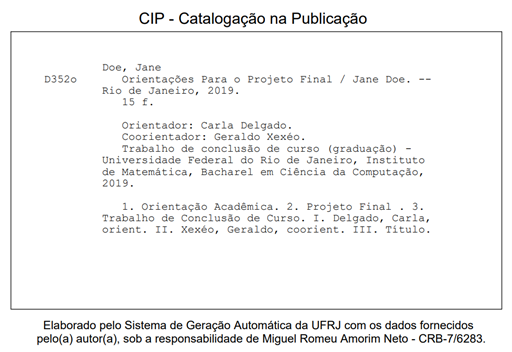
\includegraphics[width=0.9\linewidth]{imagens/ficha}
    \caption{Uma ficha catalográfica}
    \label{fig:ficha}
\end{figure}


\subsection{Resumo e Abstract}

Deve ser a última parte a ser escrita, pois só depois de completar o projeto e o texto você terá uma visão geral e poderá identificar o que é mais importante, bem como escrever com mais conhecimento de causa e maturidade. É um texto curto (entre 150 e 500 palavras) que serve para comunicar de forma bem objetiva: o que foi feito, qual a importância do que foi feito, quais os principais resultados e conclusões.

O abstract é uma tradução do mesmo texto do resumo para o inglês. Cuidado com a tradução automática, ela não dá resultados perfeitos para este tipo de texto. Revise cuidadosamente e ajuste o que ficou estranho.

\subsection{Introdução}

A seção de introdução vai fornecer ao leitor uma ideia geral do que está por vir, e motivá-lo a pensar que seu trabalho é interessante e está bem feito. Para isso, deve ser um texto leve e claro, porém informativo. Abaixo estão descritos os elementos que a introdução deve conter. Eles não precisam estar separados em seções específicas, pois muitas vezes o texto fica melhor quando não é subdividido. Tampouco estes elementos precisam aparecer necessariamente nessa ordem. Mas todos estes elementos têm que estar na introdução.

\begin{outline}
\1 Forneça o \textbf{contexto} da sua área tema, e o “estado da arte” (o que se acredita atualmente ser o melhor pra esse contexto) de forma bem resumida. Ao descrever o contexto, tente citar ao menos 3 artigos recentes que evidenciem a base conceitual na qual seu PFC estará inserido.

\1 Descreva o \textbf{problema} que o seu PFC está atacando. É mais fácil formular essa descrição identificando as perguntas que gostaríamos de responder que estão guiando o desenvolvimento do PFC. O orientador é de grande ajuda nessa parte. Na sua descrição do problema, tente citar ao menos 3 artigos científicos recentes que evidenciem a existência do problema e o descrevam.

\1 Diga porque o que vc quer fazer é importante (\textbf{justificativa}). Aqui, é interessante citar em torno de 3 artigos científicos recentes que evidenciem os impactos negativos do problema atacado.

\1 Descreva o \textbf{objetivos geral e os objetivos específicos} do seu PFC (condizentes com o item anterior). O objetivo geral é muito alinhado com a pergunta que se está tentando responder. Os objetivos específicos são desdobramentos do objetivo geral, e vão ser base para etapas do seu PFC. O esperado é que atingindo os objetivos específicos, você estará caminhando para atingir o objetivo geral.

\1 Forneça então uma descrição do que virá no resto do texto, em um parágrafo, dizendo o que aparece em cada capítulo. Algo do tipo:

\2 “Neste trabalho abordaremos estratégias para entender e implementar a volta dos que não foram. No capítulo 2 será feito um levantamento dos dados daqueles que não foram. O capítulo 3 discute a volta destas pessoas. No capítulo 4 apresentamos as estratégias levantadas e sua justificativa. No Capítulo 5 apresentamos os resultados dos testes feitos com cada estratégia. As conclusões obtidas são apresentadas no capítulo 6.“
\end{outline}

Repare que o capítulo 1 não foi mencionado propositalmente, pois se trata da própria introdução. As seções anteriores ao capítulo 1 (resumo, agradecimentos, etc) não recebem numeração de capítulo, mas tem uma formatação própria, indicada no template, como pedido pelas normas da ABNT.


\subsection{Demais capítulos}

Não há uma regra fixa que determine quantos capítulos o PFC deve ter. O número vai depender de como o texto ficará melhor organizado. Mas há coisas essenciais que devem aparecer nos capítulos seguintes.

Fundamentos. Após apresentar o seu PFC na introdução, os capítulos que vem imediatamente a seguir (um ou mais) devem trazer um resumo sobre os fundamentos nos quais você embasou o seu trabalho. Veja com seu orientador o que seriam os fundamentos, no caso do seu projeto específico.

Após os fundamentos, seguem-se capítulos sobre o “estado da arte” do que tange o problema e a solução que você está construindo para o seu PFC. O que já existe para tentar resolver o mesmo problema que você está tentando resolver? Quais as vantagens e desvantagens? Porque você resolveu tentar atacar este mesmo problema, e como você compara a sua proposta de solução com as existentes?

A seguir, os capítulos (um ou mais) devem apresentar em detalhe e com rigor a proposta do seu PFC e nos capítulos seguintes, seus desdobramentos.

Os últimos capítulos são os de resultados e conclusões (pode ser um só ou dois em separado).

\subsection{Conclusão}

O último capítulo de um trabalho acadêmico sempre apresenta as conclusões. Ele deve rever o que foi proposto e o que foi alcançado. É muito importante ressaltar o que foi obtido no PFC. Além disso, são esperadas sugestões para trabalhos futuros, principalmente se o PFC é ligado a pesquisa.

\subsection{Referências}

Dado que as carreiras estudadas nas universidades tem toda uma história já percorrida, é esperado que o aluno use seus conhecimentos para construir seu PFC sobre o que já é sabido, e não fique “reinventando a roda” e nem desperdice tempo tentando coisas que já se sabe como fazer de forma melhor ou mais eficiente. Porém, nem toda informação disponível é confiável, e é esperado que o aluno já tenha consciência disso no momento de desenvolver seu PFC.

Portanto, não apenas é essencial que o PFC tenha referências a trabalhos já consolidados, como é vital que as referências escolhidas sejam confiáveis e de qualidade. Um trabalho que traz referências duvidosas é visto duplamente com maus olhos. Primeiro porque provavelmente, como um castelo de cartas, pode “desmoronar” (não funcionar, ou chegar a conclusões falsas) por falta de fundamento adequado. Segundo, porque revela que o aluno não tem senso crítico e não sabe fazer escolhas razoáveis dentro de sua carreira. Ao escolher as fontes para referenciar em seu trabalho, selecione textos de autores consagrados, ou editados por editores sérios (ou ambas as coisas).

Livros são a fonte mais adequada para conhecimentos consolidados. Já para conhecimentos inovadores (caso seu PFC aborde temas inovadores) as referências mais adequadas são artigos científicos recentes, publicados por autores especialistas na área, em conferências e revistas organizadas por entidades sérias (ACM, IEEE, SBC, Springer, etc).

Textos de entidades empresariais e sociais podem ser referenciados, porém em casos específicos quando estas entidades (jornais tipo o globo, empresas públicas ou privadas) são as detentoras das informações que você está citando. Sites comerciais seguem as mesmas regras.

Não tem normalmente sentido usar como referência sobre um assunto de computação um artigo de uma revista de circulação comum (por exemplo, a revista super-interessante), porém podem ser usados para informar de fatos ou indicativos de interesse. Isso porque essas fontes são feitas para pessoas leigas em computação, e não há garantia que sejam editadas por especialistas.

A Wikipédia não é uma fonte científica confiável. Pode ser usada para obter informações, mas é necessário confirmá-las e citá-las pela sua origem.

Um jovem profissional da área da Ciência da Computação tem condições de ler livros e revistas científicas que forneçam uma abordagem melhor fundamentada e detalhada.

IMPORTANTE: todos os itens referenciados no PFC devem ser citados ao longo do texto. Ver no template como isso deve ser feito.
A bibliografia pode ser gerenciada por meio de vários softwares. Os dois principais disponíveis são o Zotero e o Mendeley. Uma versão mais simples, para quem usa  o LaTeX, é o JabRef.

\subsection{Apêndices e Anexos}

Em alguns trabalhos é necessário o uso de apêndices e anexos. Esses são capítulos adicionais que aparecem no fim e que servem para apresentar informações que não trariam benefícios a leitura do texto, mas são importantes.

Existe uma diferença entre apêndice e anexo: apêndices são elaborados pelo autor, anexos não são, mas podem ajudar a fundamentar, comprovar ou ilustrar o texto.

Um exemplo de informação típica de um apêndice seria o resultado de todas as respostas dadas em função de um questionário, respondente por respondente, ou listagens de código, ou provas completas de corolários de um teorema importante do trabalho.

Já um anexo poderia mostrar um mapa de uma área pesquisada, ou tabelas obtidas em algum órgão público.